\documentclass{standalone}
\usepackage{tikz}
\begin{document}
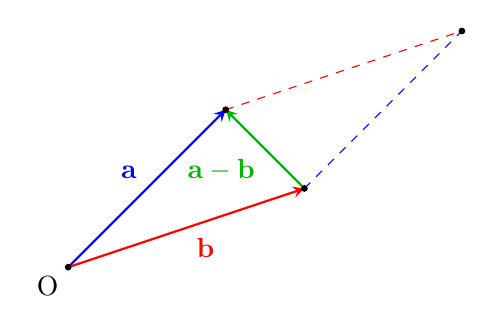
\begin{tikzpicture}[>=stealth, scale=1.0]
    % Vector a
    \draw[->, thick, blue] (0,0) -- (2,2) node[midway, above left] {${\bf a}$};
    
    % Vector b
    \draw[->, thick, red] (0,0) -- (3,1) node[midway, below right] {${\bf b}$};
    
    % Vector a + b via tip-to-tail
    \draw[dashed, red] (2,2) -- (5,3);
    \draw[dashed, blue] (3,1) -- (5,3);
    
    % Vector a - b
    \draw[->, thick, green!70!black] (3,1) -- (2,2) node[midway, below left] {${\bf a}-{\bf b}$};
    
    % Dots for clarity
    \filldraw (0,0) circle (1pt) node[below left] {O};
    \filldraw (2,2) circle (1pt);
    \filldraw (3,1) circle (1pt);
    \filldraw (5,3) circle (1pt);
\end{tikzpicture}
\end{document}